\section{Mass Action switches}

When faced with a set of competing designs for a given genetic circuit, one is likely to choose the simplest possible model that can achieve the desired behaviour. However, simple systems are often the least robust. Here we define a robust device as a device that can withstand fluctuations in parameter values and still produce the desired behaviour. Feedback loops are well known key regulatory motifs \autocite{Brandman:2005ci}. Negative feedback loops are essential for homeostasis and buffering \autocite{Thomas:1995id} thus increasing robustness to extrinsic noise sources and positive feedback loops can generate multistationarity in a system \autocite{Thomas:1995id}. Incorporating this kind of additional feedback interactions can make a design more robust and reliable. Here we use StabilityFinder to compare the robustness of two switches, a simple toggle switch and a switch with added positive auto-regulation. 
In order to study this system in the most realistic way, we avoid using the quasi-steady state approximation (QSSA) that is often used in modelling the toggle switch. The QSSA assumes that the binding/unbinding processes are much faster than any other process \autocite{Loinger:2007vma} thus the bound intermediate is assumed to always be in steady state. The QSSA is often used since it reduces the dimensions of the system thus reducing computational time \autocite{Pedersen:2007ke}. The QSSA assumption is met in vitro but often does not hold in vivo. Its misuse can lead to large errors and incorrectly estimated parameters \autocite{Pedersen:2007ke}. Parameter estimation is central to this project and since StabilityChekcker is able to analyse models with numerous equations and parameters, there is no need for this assumption, which approximates a solution. Using Mass Action, the two models used are shown below:

Standard toggle switch:
$$
\begin{array}{cccc}
      \textrm{gA}\stackrel{\textrm{ge}}{\longrightarrow}\textrm{gA} + \textrm{A} \\
      \textrm{gB}\stackrel{\textrm{ge}}{\longrightarrow}\textrm{gB} + \textrm{B} \\
      \textrm{A} + \textrm{A} \stackrel{\textrm{dim}}{\longrightarrow}\textrm{A2} \\
      \textrm{A2} \stackrel{\textrm{dim r}}{\longrightarrow}\textrm{A} + \textrm{A} \\
      \textrm{B} + \textrm{B} \stackrel{\textrm{dim}}{\longrightarrow} \textrm{B2} \\
      \textrm{B2} \stackrel{\textrm{dim\_r}}{\longrightarrow}\textrm{B} + \textrm{B} \\
      \textrm{gA} + \textrm{B2} \stackrel{\textrm{rep}}{\longrightarrow}\textrm{B2gA} \\
      \textrm{B2gA} \stackrel{\textrm{rep\_r}}{\longrightarrow}\textrm{B} + \textrm{gA} \\
      \textrm{gB} + \textrm{A2} \stackrel{\textrm{rep}}{\longrightarrow}\textrm{A2gB} \\
      \textrm{A2gB} \stackrel{\textrm{rep\_r}}{\longrightarrow}\textrm{A2} + \textrm{gB} \\
      \textrm{A} \stackrel{\textrm{deg}}{\longrightarrow}\textrm{\O}\\
      \textrm{B} \stackrel{\textrm{deg}}{\longrightarrow}\textrm{\O}\\
      \textrm{S} + \textrm{A2} \stackrel{\textrm{rep\_dim}}{\longrightarrow}\textrm{SA2}\\
      \textrm{SA2} \stackrel{\textrm{rep\_dim\_r}}{\longrightarrow}\textrm{S} + \textrm{A2}\\
      \textrm{R} + \textrm{B2} \stackrel{\textrm{rep\_dim}}{\longrightarrow}\textrm{RB2}\\
      \textrm{RB2} \stackrel{\textrm{rep\_dim\_r}}{\longrightarrow}\textrm{R} + \textrm{B2}\\
      \textrm{R} \stackrel{\textrm{deg}}{\longrightarrow} \textrm{\O}\\
      \textrm{S} \stackrel{\textrm{deg}}{\longrightarrow}\textrm{\O}\\
\end{array}
$$

Double positive autoregulation:
$$
\begin{array}{cccc} 
    \textrm{A2} + \textrm{gA} \stackrel{\textrm{aut 1}}{\longrightarrow} \textrm{A2gA} \\
    \textrm{A2gA} \stackrel{\textrm{aut 2}}{\longrightarrow} \textrm{A} + \textrm{A2gA}\\
    \textrm{A2gA} \stackrel{\textrm{aut 3}}{\longrightarrow} \textrm{A2}+ \textrm{gA}  \\
    \textrm{B2} + \textrm{gB} \stackrel{\textrm{aut 1}}{\longrightarrow} \textrm{B2gB} \\
    \textrm{B2gB} \stackrel{\textrm{aut 2}}{\longrightarrow} \textrm{B} + \textrm{B2gB}\\
    \textrm{B2gB} \stackrel{\textrm{aut 3}}{\longrightarrow} \textrm{B2}+ \textrm{gB}  \\
\end{array}
$$

\subsection{Deterministic case}
\subsubsection{Symmetric switch}
Using the same priors for their shared parameters, we used StabilityFinder for both models in order to compare their robustness. The corresponding posterior distributions can be seen in Figures~\ref{fig:det_std} and ~\ref{fig:doub_pos}.

\begin{table}[p]
\centering
\caption{Mass Action switches priors}
\label{tab:simp}
\begin{tabular}{cccccccccc}
ge   & rep  & rep\_r & dim  & dim\_r & deg & deg\_dim & aut\_1 & aut\_2 & aut\_3\\
1-10 & 1-10 & 1-10    & 1-10 & 0-5    & 1-10 & 0-0.5   &1-10&5-10&1-5
\end{tabular}
\end{table}


\begin{figure}[p]
\centering
\includegraphics[scale=0.2]{chapterModelling/mass_action_switches/deterministic/posterior_ma_cl_bi.png}
\caption{The posterior distribution of the mass action simple toggle switch}
\label{fig:det_std}
\end{figure}

\begin{figure}[p]
\centering
\includegraphics[scale=0.3]{chapterModelling/mass_action_switches/deterministic/ma_cl_bi_phase_plot.png}
\caption{A sample of the phase plots produced from the final population of the mass action simple toggle switch.}
\label{fig:det_std_phase}
\end{figure}

\begin{figure}[p]
\centering
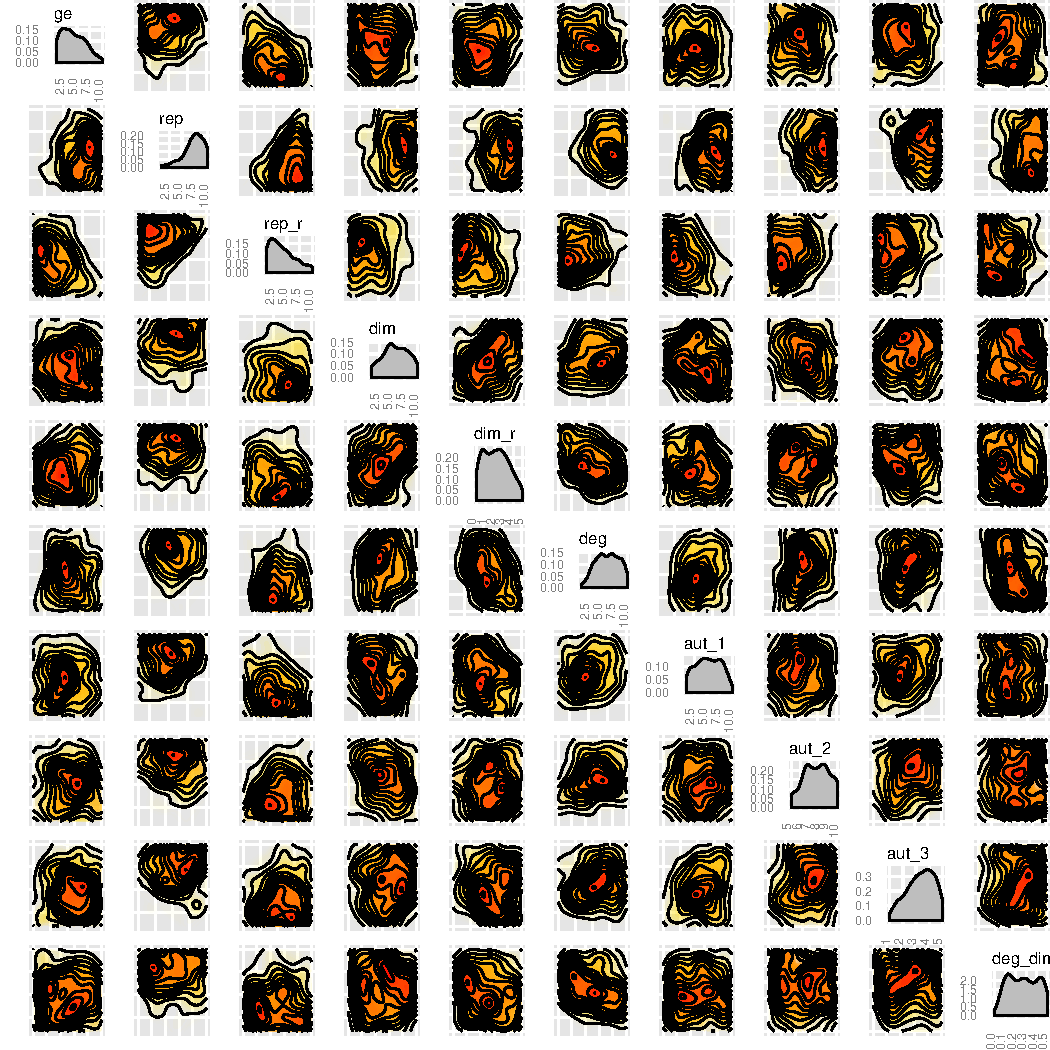
\includegraphics[scale=0.2]{chapterModelling/mass_action_switches/deterministic/posterior_ma_dp_bi.png}
\caption{The posterior distribution of the Mass action double positive feedback loop switch}
\label{fig:doub_pos}
\end{figure}

\begin{figure}[p]
\centering
\includegraphics[scale=0.3]{chapterModelling/mass_action_switches/deterministic/ma_dp_bi_phase_plot.png}
\caption{A sample of the phase plots produced from the final population of the mass action double positive feedback toggle switch.}
\label{fig:det_dp_phase}
\end{figure}

In order to directly compare the robustness of the two models, we used the algorithm outlined in the Methods as a measure of how wide each posterior is given the priors. The results are shown in Figure~\ref{fig:robust_std_doubpos}. 

\begin{figure}[h]
\centering
\includegraphics[scale=0.5]{chapterModelling/mass_action_switches/deterministic/MA_robustness_cartoon.png}
\caption[The robustness of the double positive and the simple switch mass action models]{The switch with double positive autoregulation is more robust to parameter fluctuations that the simple switch. This is evident from the fact that the switch with added feedback has a larger posterior distribution under which it is bistable, compare to the simple switch. Robustness was calculated using a Monte Carlo accept reject algorithm. }
\label{fig:robust_std_doubpos}
\end{figure}
As seen in Figure~\ref{fig:robust_std_doubpos}, the toggle switch with double positive autoregulation is more robust than the simple switch with no feedback. Adding positive feedback loops to the model allows it to be bistable over a greater range of parameter values. This indicates that small fluctuations in parameters in the cellular environment will not flip the switch and thus makes it more suitable for use in synthetic biological applications where spontaneous and undesired switching might be detrimental. 
\clearpage

\subsubsection{Asymmetric switch}
Next, we studied the asymmetric model of the deterministic mass action switch. In this model there are separate gene expression and repression parameters for each gene. The priors used were the ones shown in Table~\ref{tab:asym_cl_det_ma}. The posterior obtained for the classical case is shown in Figure~\ref{fig:asym_det_cl_ma_post} and for the double positive case in Figure~\ref{fig:asym_det_dp_ma_post}.

\begin{table}[htbp]
\centering
\caption{Deterministic asymmetric Mass Action switch priors}
\label{tab:asym_cl_det_ma}
\begin{tabular}{cc}
parameter & range \\
geA & 5-10 \\
repA & 2-10 \\
rep\_r & 0-5 \\
dim & 5-10 \\
dim\_r & 0-5 \\
deg & 1-5 \\
deg\_dim & 0-0.1 \\
geB & 5-10 \\
repB & 2-10 \\
aut\_1 & 1-10\\
aut\_2 & 5-10\\
aut\_3 & 1-5\\
\end{tabular}
\end{table}

\begin{figure*}[htbp]
\begin{center}
\includegraphics[scale=0.15]{chapterModelling/mass_action_switches/deterministic/asym/posterior_cl.png}
\caption{Posterior of simple asymmetric deterministic switch}\label{fig:asym_det_cl_ma_post}
\end{center}
\end{figure*}

\begin{figure*}[htbp]
\begin{center}
\includegraphics[scale=0.15]{chapterModelling/mass_action_switches/deterministic/asym/cl_det_phase.png}
\caption{Phase plot of simple asymmetric deterministic switch}\label{fig:asym_det_cl_ma_phase}
\end{center}
\end{figure*}

\begin{figure*}[htbp]
\begin{center}
\includegraphics[scale=0.1]{chapterModelling/mass_action_switches/deterministic/asym/posterior_dp.png}
\caption{Posterior of double positive asymmetric deterministic switch}\label{fig:asym_det_dp_ma_post}
\end{center}
\end{figure*}

\begin{figure*}[htbp]
\begin{center}
\includegraphics[scale=0.2]{chapterModelling/mass_action_switches/deterministic/asym/dp_det_phase.png}
\caption{Phase plot of double positive asymmetric deterministic switch}\label{fig:asym_det_dp_ma_phase}
\end{center}
\end{figure*}

\clearpage
\subsubsection{Including transcription and translation}
In order to make these models more realistic, we also separated transcription from translation steps. This is done by adding two parameters to the model to represent translation, while the parameters for gene expression now represent only transcription. The priors used were the ones shown in Table~\ref{tab:asym_cl_rna_det_ma}. The posterior obtained for the classical case is shown in Figure~\ref{fig:asym_det_cl_rna_ma_post} and for the double positive case in Figure~\ref{fig:asym_det_dp_rna_ma_post}.

\begin{table}[htbp]
\centering
\caption{Deterministic asymmetric Mass Action RNA switch priors}
\label{tab:asym_cl_rna_det_ma}
\begin{tabular}{cc}
parameter & range \\
geA & 5-10 \\
trnslA & 0-10 \\
trnslB & 0-10 \\
repA & 2-10 \\
rep\_r & 0-5 \\
dim & 5-10 \\
dim\_r & 0-5 \\
deg & 1-5 \\
deg\_dim & 0-0.1 \\
geB & 5-10 \\
repB & 2-10 \\
aut\_1 & 0-10\\
aut\_2 & 0-10\\
aut\_3 & 0-1\\
\end{tabular}
\end{table}

\begin{figure*}[htbp]
\begin{center}
\includegraphics[scale=0.15]{chapterModelling/mass_action_switches/deterministic/asym/posterior_cl_rna.png}
\caption{Posterior of simple asymmetric RNA deterministic switch}\label{fig:asym_det_cl_rna_ma_post}
\end{center}
\end{figure*}


%\begin{figure*}[htbp]
%\begin{center}
%\includegraphics[scale=0.2]{chapterModelling/mass_action_switches/deterministic/asym/rna_cl_det_phase.png}
%\caption{Phase plot of simple asymmetric RNA deterministic switch}\label{fig:asym_det_cl_rna_ma_phase}
%\end{center}
%\end{figure*}


\begin{figure*}[htbp]
\begin{center}
\includegraphics[scale=0.15]{chapterModelling/mass_action_switches/deterministic/asym/posterior_dp_rna.png}
\caption{Posterior of double positive asymmetric RNA deterministic switch}\label{fig:asym_det_dp_rna_ma_post}
\end{center}
\end{figure*}

%\begin{figure*}[htbp]
%\begin{center}
%\includegraphics[scale=0.2]{chapterModelling/mass_action_switches/deterministic/asym/rna_dp_det_phase.png}
%\caption{Phase plot of double positive asymmetric RNA deterministic switch}\label{fig:asym_det_dp_rna_ma_phase}
%\end{center}
%\end{figure*}



\clearpage


%-----%-----%-----%-----%
\subsection{Stochastic case}
\subsubsection{Bistable} 
The model consists of asymetric parameters for gene expression and repression. We search for the parameter space that makes this model tristable. Example phase plots of the resulting tristable switches are shown below. 1000 particles were used in these simulations.


\begin{table}[htbp]
\centering
\caption{priors of bistable switches}
\label{tab:priors_bi}
\begin{tabular}{cc}
parameter & range \\
geA & 0-10 \\
repA & 0-10 \\
rep\_r & 0-10 \\
dim & 7-15 (0-20 in double pos)\\
dim\_r & 0-10 \\
deg & 0-10 \\
deg\_dim & 0-1 \\
geB & 0-10 \\
repB & 0-10 \\
aut\_1 & 0-10 \\
aut\_2 & 0-10 \\
aut\_3 & 0-10
\end{tabular}
\end{table}

\begin{figure*}[htbp]
\begin{center}
\includegraphics[scale=0.2]{chapterModelling/mass_action_switches/bi_stoch_images/phase_plt.png}
\caption{Phase plot of the bistable switch.}\label{fig_5}
\end{center}
\end{figure*}

The posterior distributions of the two swicthes:

\begin{figure*}[htbp]
\begin{center}
\includegraphics[scale=0.15]{chapterModelling/mass_action_switches/bi_stoch_images/posterior_std.png}
\caption{Posterior of simple switch}\label{fig_6}
\end{center}
\end{figure*}

\begin{figure*}[htbp]
\begin{center}
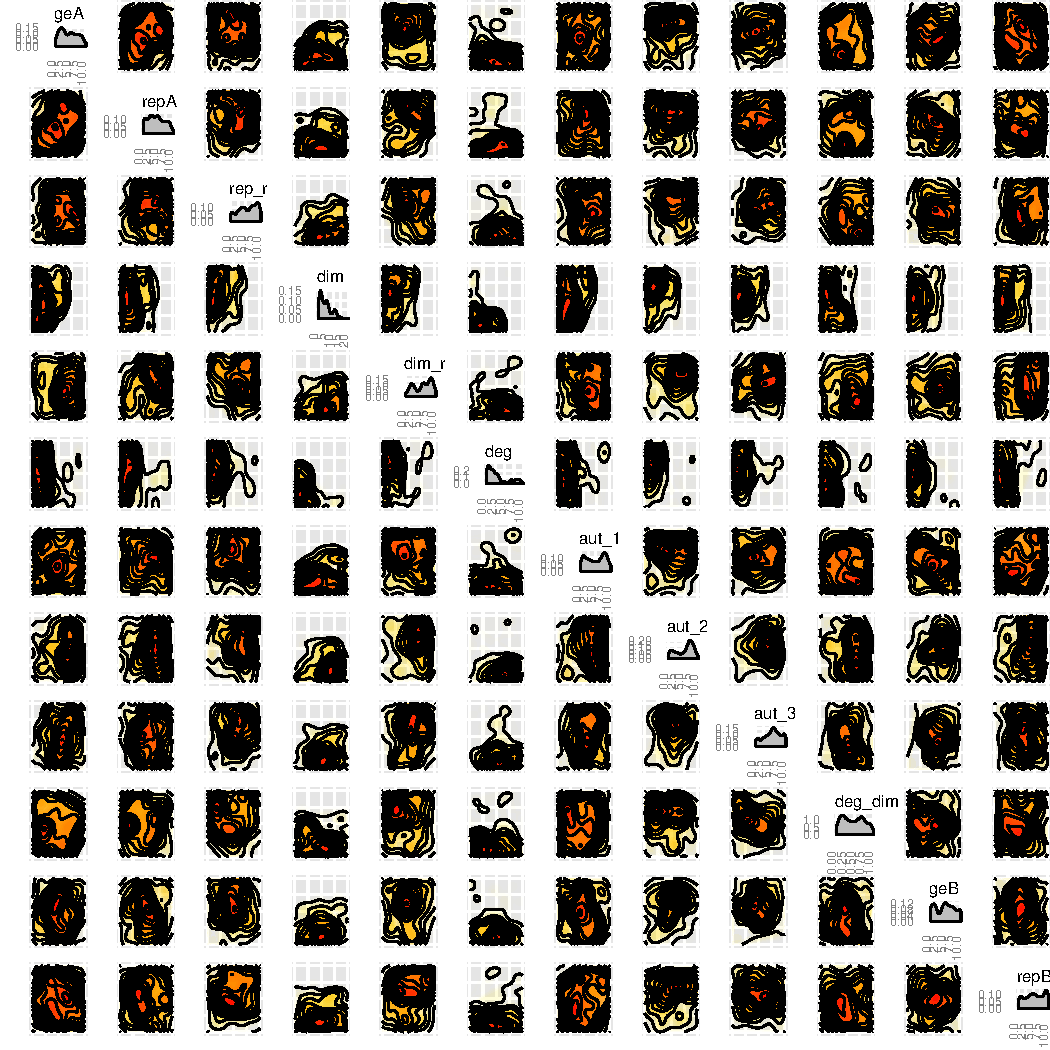
\includegraphics[scale=0.15]{chapterModelling/mass_action_switches/bi_tri_same_priors/posterior_pos_ab_bi.png}
\caption{Posterior of switch with double positive autoregulation}\label{fig_7}
\end{center}
\end{figure*}

%The robustness of the two switches was compared and no difference was found between the two:
%\newpage
%\begin{figure*}[h!]
%\begin{center}
%\includegraphics[scale=0.7]{chapterModelling/mass_action_stochastic_switches/bi_stoch_images/robustness_comparison.pdf}
%\caption{Robustness comparison of the bistable switches. There is no significant diffrence between the two.}\label{fig_8}
%\end{center}
%\end{figure*}

\clearpage
\subsubsection{Tristable}
The model consists of asymmetric parameters for gene expression and repression. We search for the parameter space that makes this model tristable. Example phase plots of the resulting tristable switches are shown below. 1000 particles were used in these simulations.
 
 \begin{table}[htbp]
\centering
\caption{priors of tristable switches}
\label{tab:priors_tri}
\begin{tabular}{cc}
parameter & range \\
geA & 0-10 \\
repA & 0-10 \\
rep\_r & 0-10 \\
dim & 0-20 \\
dim\_r & 0-10 \\
deg & 0-10 \\
deg\_dim & 0-1 \\
geB & 0-10 \\
repB & 0-10 \\
aut\_1 & 0-10 \\
aut\_2 & 0-10 \\
aut\_3 & 0-10
\end{tabular}
\end{table}

\begin{figure*}[h!]
\begin{center}
\includegraphics[scale=0.2]{chapterModelling/mass_action_switches/tri_stoch_images/phase_plot_tri.png}
\caption{Phase plot of the tristable switch.}\label{fig_1}
\end{center}
\end{figure*}

The posterior distributions of the two switches:

\begin{figure*}[htbp]
\begin{center}
\includegraphics[scale=0.15]{chapterModelling/mass_action_switches/bi_tri_same_priors/posterior_std_tri.png}
\caption{Posterior of simple switch}\label{fig_2}
\end{center}
\end{figure*}

\begin{figure*}[htbp]
\begin{center}
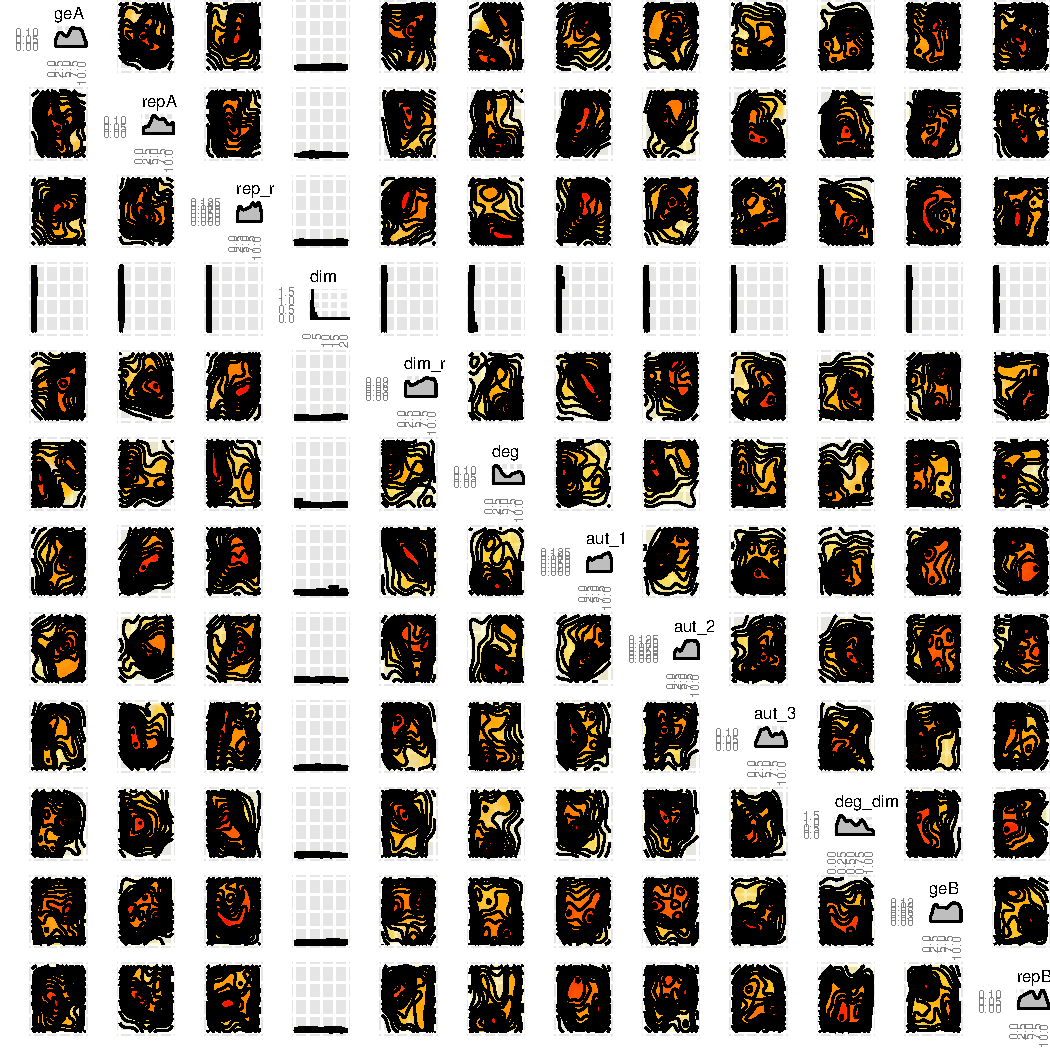
\includegraphics[scale=0.15]{chapterModelling/mass_action_switches/bi_tri_same_priors/posterior_pos_ab_tri.png}
\caption{Posterior of switch with double positive autoregulation}\label{fig_3}
\end{center}
\end{figure*}
\clearpage
It is clear that in both cases of the switch, the parameter for dimerisation (dim) is very constrained to low values. On the other and, the values for the reverse reaction, the unbinding of dimerisation is not constrained and can take up larger values. 

The robustness of the two switches was compared and no difference was found between the two:

\begin{figure*}[h!]
\begin{center}
\includegraphics[scale=0.1]{chapterModelling/mass_action_switches/bi_tri_same_priors/robustness_comparison_tri.png}
\caption{Robustness comparison of the tristable switches. There is no significant difference between the two.}\label{fig_4}
\end{center}
\end{figure*}
\clearpage

\subsubsection{Extracting the design principles of a tristable switch}
Next, we went on to study the design principles that make a switch tristable vs bistable. To do this we implemented an algorithm, as shown in the Appendix. Samples were taken from the posterior distribution of the stochastic double positive mass action tristable switch. Then we separated the values that, for each parameter, were also found in the posterior of the bistable switch. The same procedure was done but taking samples from the bistable posterior and looking for them in the tristable posterior. This can give an indication of the separation of parameter values that can give rise to a bistable vs a tristable switch. The results are shown in Figure ~\ref{fig:design_pr_ma_dp}.

\begin{figure*}[h!]
\begin{center}
\includegraphics[scale=0.2]{chapterModelling/mass_action_switches/bi_tri_same_priors/design_principles_pos_ab.png}
\caption{Extracting the tristable versus bistable switch design principles. Yellow represents a bistable switch and red a tristable}\label{fig:design_pr_ma_dp}
\end{center}
\end{figure*}

From the above results it can be seen that the only parameter that is different in the two switches is the one representing dimerisation (dim). For both a bistable and a tristable switch the value for dim must be small, although this condition is more constrained in a tristable switch.
